\section{Illustration of Phase 1}
\label{app:phase1}   
Figures \ref{img:phase1img1} -- \ref{img:phase1img13} illustrates the construction of the weight coefficients set $\Q$ for the Eisenstein base $\beta = -\frac{3}{2} + \frac{\imath \sqrt{3}}{2}$ with the complex alphabet $\mathcal{A} =\{0, 1, -1, \omega, -\omega, -\omega - 1, \omega + 1\}$(see Example \ref{ex:Eisenstein1-blockcomplex}).

\figurehascaptionOne{1 = The starting set $\Q_0{=}\{0\}$.}
\figurehascaptionOne{2 = The set $\B+\Q_0$ need to be covered.}
\figurehascaptionOne{3 = The set $\Q_0$ does not cover the set $\B+\Q_0${,} i.e.{,} the set $\A+\beta \cdot \Q_0$ is not superset of $\B+\Q_0$.}
\figurehascaptionOne{4 = The set $\Q_0$ is extended to $\Q_1$ to cover all elements of $\B+\Q_0$.}
\figurehascaptionOne{5 = The set $\B+\Q_1$ need to be covered.}
\figurehascaptionOne{6 = The set $\Q_1$ does not cover the set $\B+\Q_1${,} i.e.{,} the set $\A+\beta \cdot \Q_1$ is not superset of $\B+\Q_1$.}
\figurehascaptionOne{7 = The set $\Q_1$ is extended to $\Q_2$ to cover all elements of $\B+\Q_1$.}
\figurehascaptionOne{8 = The set $\B+\Q_2$ need to be covered.}
\figurehascaptionOne{9 = The set $\Q_2$ does not cover the set $\B+\Q_2${,} i.e.{,} the set $\A+\beta \cdot \Q_2$ is not superset of $\B+\Q_2$.}
\figurehascaptionOne{10 = The set $\Q_2$ is extended to $\Q_3$ to cover all elements of $\B+\Q_2$.}
\figurehascaptionOne{11 = The set $\B+\Q_3$ need to be covered.}
\figurehascaptionOne{12 = The set $\Q_3$ covers the set $\B+\Q_3${,} i.e.{,} the set $\A+\beta \cdot \Q_3$ is superset of $\B+\Q_2$.}
\figurehascaptionOne{13 = The final weight coefficients $\Q{=}\Q_3$.}


\foreach \n in {1,...,13} {%
\begin{SCfigure}[][htbp]
    \centering
    \caption{\getcaptionOne{\n}}
    \label{img:phase1img\n}
    \includegraphics[height=0.3\textheight]{img/eisenstein/phase1_image_\n.png}
\end{SCfigure}
    }

\newpage
\figurehascaptionTwo{1 = Phase 2 starts with the weight coefficients set $\Q$ from Phase 1.}
\figurehascaptionTwo{2 = The set $\omega+\Q$ need to be covered.}
\figurehascaptionTwo{3 = The elements of $\omega+\Q$ are covered by the set $\Q_{[\omega]}$.}
\figurehascaptionTwo{4 = The set $\omega+\Q_{[1]}$ need to be covered.}
\figurehascaptionTwo{5 = The elements of $\omega+\Q_{[1]}$ are covered by the set $\Q_{[\omega,1]}$.}
\figurehascaptionTwo{6 = The set $\omega+\Q_{[1,2]}$ need to be covered.}
\figurehascaptionTwo{7 = The elements of $\omega+\Q_{[1]}$ are covered by the set $\Q_{[\omega,1,2]}$ which has only one element{.} This element is the output of the weight function $q{(\omega,1,2)}$.}


\section{Illustration of Phase 2}
The construction of set $\Q_{[\omega,1,2]}$ for the Eisenstein base $\beta = -\frac{3}{2} + \frac{\imath \sqrt{3}}{2}$ with the complex alphabet $\mathcal{A} =\{0, 1, -1, \omega, -\omega, -\omega - 1, \omega + 1\}$ is illustrated on Figures \ref{img:phase2img1} -- \ref{img:phase2img7} (see Example \ref{ex:Eisenstein1-blockcomplex}).
\label{app:phase2}    

\foreach \n in {1,...,7} {%
\begin{SCfigure}[][htbp]
    \centering
    \caption{\getcaptionTwo{\n}}
    \label{img:phase2img\n}
    \includegraphics[height=0.3\textheight]{img/eisenstein/phase2_image_\n.png}
\end{SCfigure}
    }
    


\newpage
\section{Sample of input file for shell}
File \verb+input_sample.sage+:
\label{app:inputSample}

\lstinputlisting[language=Python]{input_sample.sage}

\section{GUI in SageMath Cloud}
\label{app:interact}
\begin{figure}[!htbp]
  \centering
  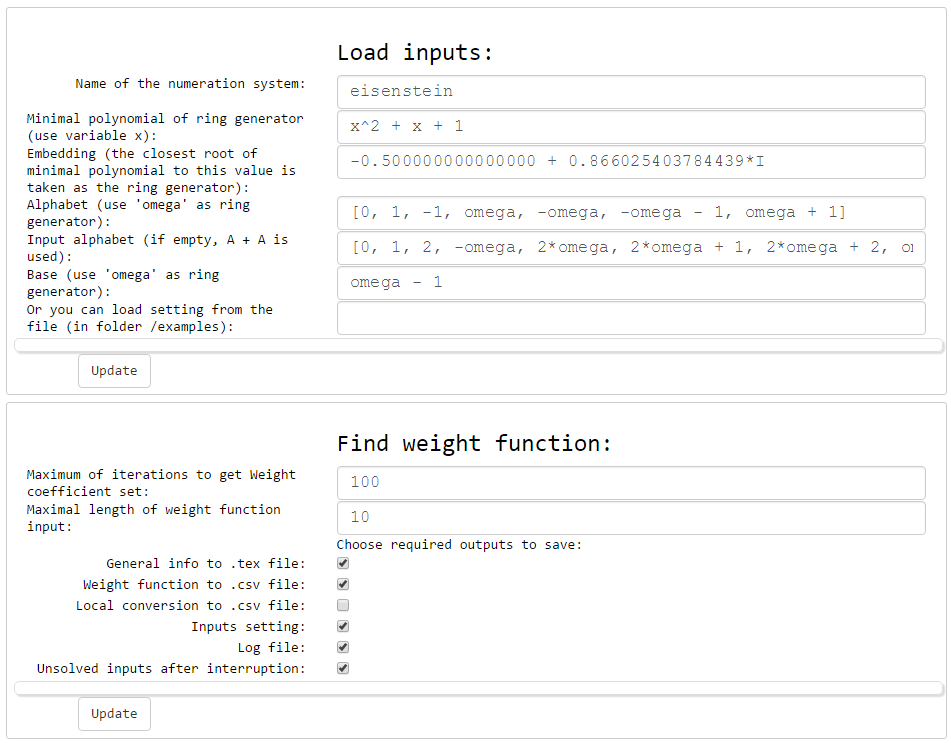
\includegraphics[width=\textwidth]{img/interact1.png}
  \caption{The graphic user interface after loading inputs.}
  \label{fig:interact1}
\end{figure}

\begin{figure}[htbp]
  \centering
  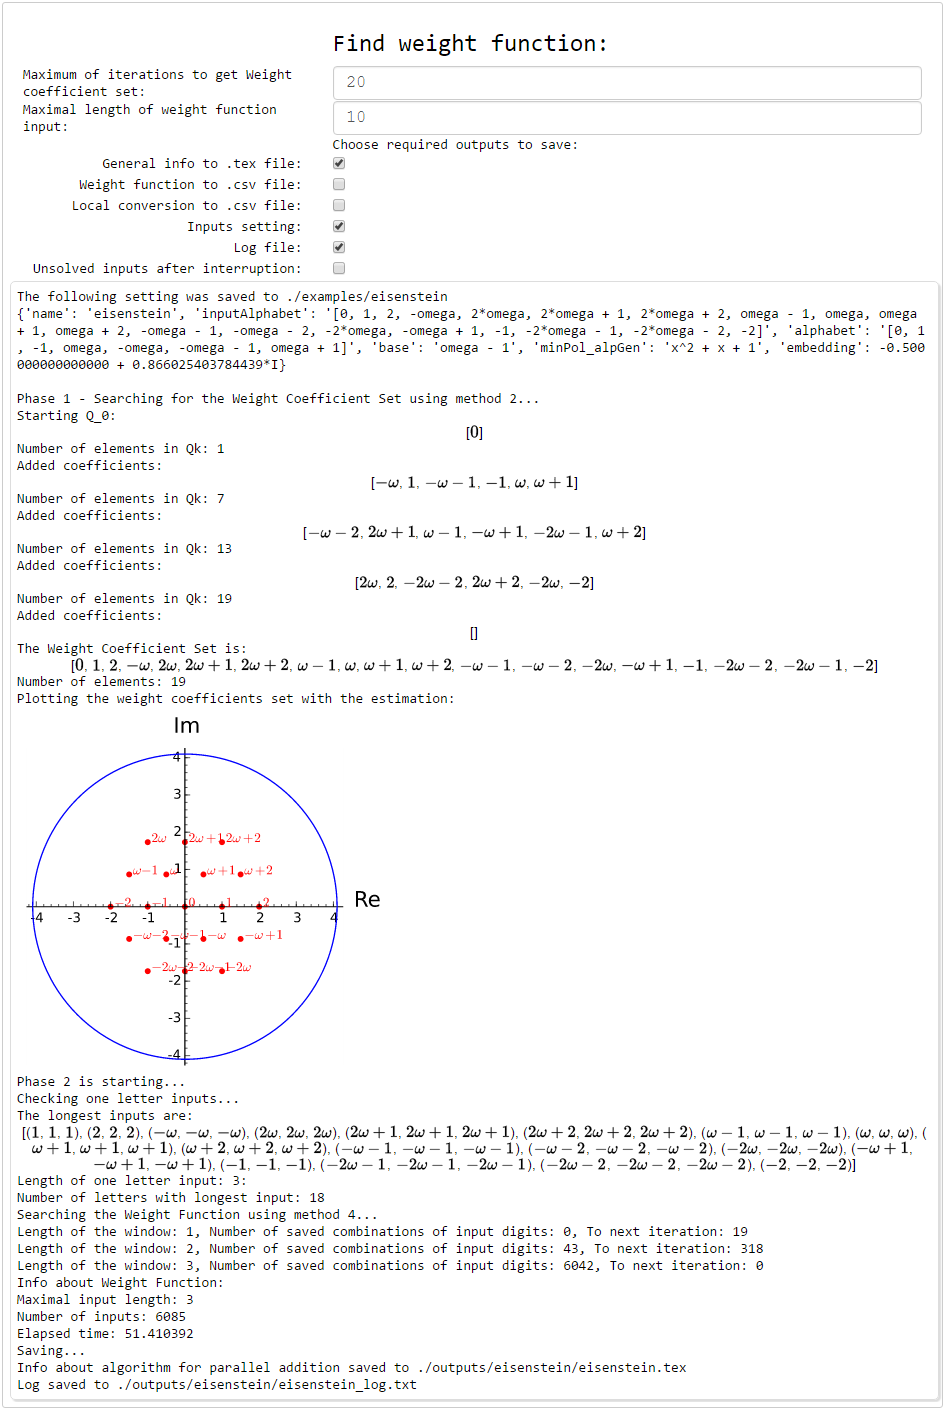
\includegraphics[width=\textwidth]{img/interact2.png}
  \caption{The output of the extending window method in the graphic user interface.}
  \label{fig:interact2}
\end{figure}

\begin{figure}[htbp]
  \centering
  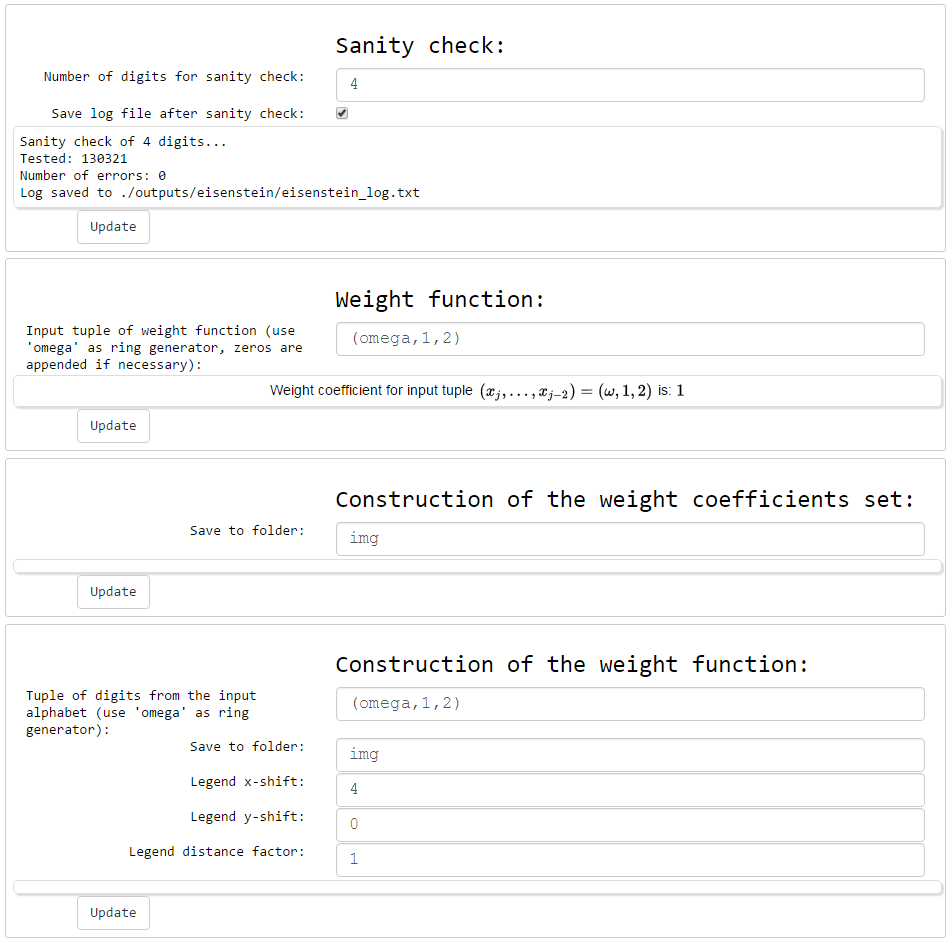
\includegraphics[width=\textwidth]{img/interact3.png}
  \caption{The part of the graphic user interface for the sanity check, calling of the weight function and plotting of images of steps of both phases.}
  \label{fig:interact3}
\end{figure}